% !TeX root = protokoll.tex
\PassOptionsToPackage{titlesec}{newparttoc}
\documentclass[ngerman,leqno,x11names]{uol-physics-report}

\partner{Hendrik Philip}{Gorka}{hendrik.philipp.gorka@uni-oldenburg.de}{6478477}
\partner{Jan Eike}{Suchard}{jan.eike.suchard@uni-oldenburg.de}{5945617}
\partner{Terje}{Zirks}{terje.zirks@uni-oldenburg.de}{6417547}
\group{2}
\module{phy215}{Grundpraktikum Physik \rom{2} -- für 2-Fach-Bachelor}
\semester{Sommersemester 2023}
\tutor{Christoph Plaßmeyer}
\supervisor{Marcel Behrens}

\makeatletter
\@addtoreset{section}{part}
\makeatother 

\usepackage{menukeys}
\usepackage{csquotes}
\usepackage{biblatex}
\usepackage{listings}
\usepackage{subcaption}
\usepackage{enumitem}
\usepackage{tcolorbox}
\usepackage{xcolor}
\usepackage{tabularx}
\usepackage{subfiles}

\captionsetup{font=footnotesize, format=hang}

\addbibresource{../global-sources.bib}
\addbibresource{sources.bib}

\graphicspath{{./images/}}
\sisetup{output-open-uncertainty = [, output-close-uncertainty = ], 
uncertainty-separator = \,}

\newenvironment{question}[2]
{
    \begin{tcolorbox}[adjusted title=\textbf{Zu Frage #1}]
        \begin{center}
            #2
        \end{center}
    \tcblower}
{
\end{tcolorbox}
}

\newtcolorbox{messageBox}[3][]
{
  colframe = #2!25,
  colback  = #2!10,
  coltitle = #2!20!black,  
  title    = {#3},
  #1,
}

\tcbset{colback=white,colframe=Maroon0, coltitle=white}


\usepackage{isotope}

\title{Abstands- und Abschwächungsgesetz für $\beta$- und $\gamma$-Strahlung}
\date{24.04.2023}

\begin{document}
\maketitle

\subfile{parts/einleitung.tex}
\newpage
\subfile{parts/theorie.tex}
\newpage
\part{Versuche}
\subfile{parts/versuch1.tex}
\newpage
\subfile{parts/versuch2.tex}
\newpage
\subfile{parts/versuch3.tex}
\newpage
\subfile{parts/versuch4.tex}
\newpage
\part{Anhang}
\printbibliography[heading=bibnumbered,title=Referenzen und Literatur]
\newpage
\section{Messwerttabelle}
Die Messwerttabelle befindet sich auf den folgenden Seiten.
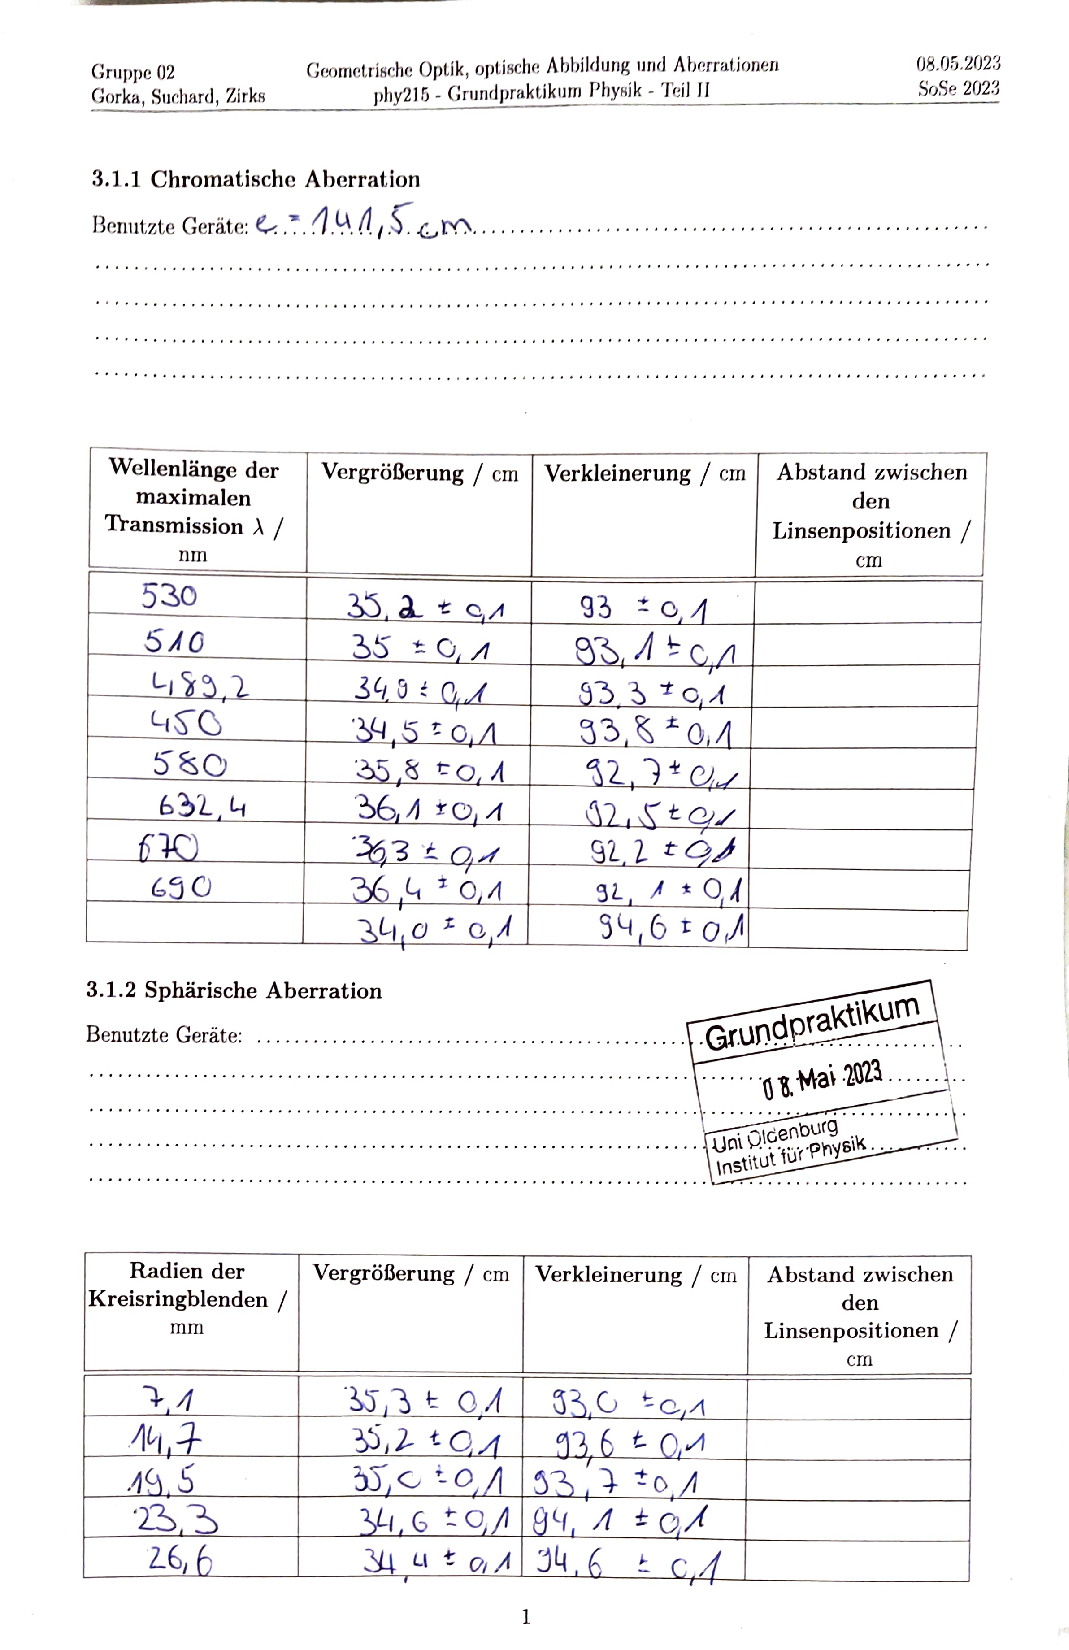
\includepdf[pages=-]{messwerttabelle.pdf}
\end{document}